\newpage
\chapter{СЖАТИЕ ВИДЕОДАННЫХ С ИСПОЛЬЗОВАНИЕМ ПРИНЦИПОВ КОДИРОВАНИЯ ЗАВИСИМЫХ ИСТОЧНИКОВ}
\label{chap1}

\section{Вводные замечания}

В течение последних десятилетий наблюдается существенное развитие технологий беспроводного обмена информацией. Пропускная способность существующих беспроводных сетей передачи данных позволяет осуществлять передачу по ним таких объемных данных как видеоданные. Следует отметить, что все чаще в современных сетях передачи данных в качестве источников такой информации выступают мобильные устройства, которые, как правило, характеризуются малыми вычислительными возможностями (при этом ограничения накладываются как на вычислительную мощность процессора, так и на доступный объем памяти) и ограниченным, зачастую трудно восполняемым, запасом аккумуляторной батареи. Существующие технологии сжатия видеоданных, в первую очередь подходы, описанные в стандартах серий ITU-T H.26x и ISO/IEC MPEG~\cite{Richardson}, характеризуются наличием «сложного» кодера и «простого» декодера, и плохо подходят для использования на мобильных устройствах. В качестве перспективной технологии для использования на мобильных устройствах во многих работах рассматриваются подходы, связанные с \textit{распределенным кодированием видеоданных} (Distributed Video Coding~--~DVC)~\cite{2397}.

Большинство современных видеокодеков используют следующую схему устранения временной избыточности: сжатию подвергаются не данные исходного кадра, а ошибки предсказания. Предсказание пикселей текущего кадра осуществляется по данным одного или нескольких ранее обработанных и уже восстановленных (декодированных) кадров. Такие кадры называют \textit{опорными} или \textit{базовыми}. Процедура поиска в опорных кадрах пикселей, которые будут использоваться для предсказания, называется \textit{оценкой движения} (Motion Estimation~--~ME), причем эта процедура может занимать до $70$\% от общего времени кодирования~\cite{5089121}.

В схемах на основе DVC устранение временной избыточности также осуществляется с помощью предсказания, однако оно выполняется на стороне декодера, что позволяет существенно снизить сложность кодирования. С точки зрения распределенного кодирования результат предсказания на стороне декодера является \textit{дополнительной информацией}, а саму процедуру предсказания называют \textit{генерацией дополнительной информации}. Кодеру остается только сформировать уточняющую информацию, которая позволит декодеру исправить ошибки предсказания. Существующие реализации DVC используют для исправления ошибок предсказания методы помехоустойчивого кодирования. Наиболее популярным подходом является интерпретация предсказания с помощью так называемого \textit{виртуального канала} (Virtual Dependency Channel), по которому <<передаются>> исходные данные $\mathbf{x}$, а на выходе наблюдается дополнительная информация (результаты предсказания) $\mathbf{y}$. Для того чтобы исправить возникшие <<ошибки>>, кодер интерпретирует $\mathbf{x}$ как информационную последовательность и формирует по ней проверочные символы, используя заранее определенный код. Декодер конкатенирует полученные проверочные символы с $\mathbf{y}$, после чего применяет процедуру декодирования, восстанавливая в $\mathbf{y}$ несовпадающие с $\mathbf{x}$ позиции. Таким образом, сжатие достигается в том случае, если количество проверочных символов меньше, чем количество исходных данных $\mathbf{x}$. Следует отметить, что описанный подход является только одним из способов практической реализации идеи DVC. Альтернативные способы будут рассмотрены в данном разделе далее.

В данной работе рассматривается процесс сжатия видеопоследовательностей с использованием методов распределенного кодирования источников. Для краткости изложения будем далее в тексте называть кодеки видеоданных, основанные на распределенном кодировании источников, \textit{распределенным кодеками видеоданных} или, если это не будет вызывать неоднозначности, просто \textit{распределенным кодеками}.

Данный раздел организован следующим образом. В начале приводится краткое введение в теорию распределенного кодирования источников. Затем вводятся основные понятия, характерные для такой системы обработки информации, и дается ряд иллюстративных примеров для пояснения ключевых идей, используемых при сжатии данных в подобных системах. Далее вводится классификация методов распределенного кодирования видеоданных и рассматриваются две базовые концепции, лежащие в основе существующих алгоритмов сжатия с использованием данного подхода. После этого вводится в рассмотрение модель распределенного кодирования на базе проекта DISCOVER, рассматриваются способы практической реализации основных модулей системы сжатия, использующей эту модель. Описание распределенного кодирования заканчивается перечислением основных прикладных задач, в которых подобный подход может использоваться.

Перед тем как переходить к дальнейшему изложению, приведем краткое описание используемых в данной работе обозначений. 
\begin{itemize}
  \item Скаляры~--~символы, набранные в нижнем регистре, например $p$.
  \item Векторы~--~символы, набранные в нижнем регистре с полужирным начертанием, например $\mathbf{a} = (a_1,a_2,...,a_n)$ задает вектор в $n$-мерном пространстве. Для определенности будем полагать, что векторы представляют собой векторы-столбцы. В таком случае вектор-строку будем определять с использованием операции транспонирования, например $\mathbf{a}^T$.
  \item Матрицы~--~символы, набранные в верхнем регистре с полужирным начертанием, например $\mathbf{A}$. Элемент, находящийся матрице $\mathbf{A}$ в строке с номером $k$ и столбце с номером $l$ будем обозначать в зависимости от контекста либо через $\mathbf{A}[k,l]$, либо через $a_{k,l}$.
  \item Случайные величины~--~символы, набранные в верхнем регистре, например $X$.
  \item Множества~--~символы, набранные в верхнем регистре курсивом, например $\mathcal{X}$. Там, где это возможно, будем задавать множества перечислением их элементов или указанием условия, которому удовлетворяют все элементы, например:
  \begin{itemize}
    \item $\mathcal{X}=\{1,2,...,q\}^m$ задает множество $q$-ичных векторов в $m$-мерном пространстве;
    \item $\mathcal{Y}=\{(i,j) \vert i \in \mathcal{R}^2, i^2+j^2<r^2\}$ содержит множество всех точек вещественной плоскости, лежащих внутри окружности радиуса~$r$.
  \end{itemize}
\end{itemize}

Для того, чтобы избежать неоднозначности, при использовании верхних индексов будут использоваться скобки, например $a^{(i)}$.
Данная система обозначений будет применяться далее в течение всего изложения.

Материал раздела изложен в работах~\cite{VeselovMonograph},~\cite{Priborostroenie2013}.

\section{Теоретические предпосылки распределенного видеокодирования}\label{chap1:HistoricalReview}

Методы распределенного кодирования видеоданных основаны на задаче кодирования зависимых источников без памяти. Эта задача, также известная как \emph{распределенное кодирование зависимых источников} (Distributed Source Coding), была впервые сформулирована и решена в работе~\cite{Slepian1973}, где была рассмотрена система передачи информации (рисунок~\ref{fig:SWSystem}) с парой зависимых дискретных источников без памяти $U_X$ и $U_Y$, на выходе которых наблюдаются ансамбли сообщений из $\mathcal{X}$ и $\mathcal{Y}$ соответственно, причем
\begin{equation*}
p(\mathbf{x},\mathbf{y}) = \prod\limits_{i=1}^{n} p(x_i,y_i),
\end{equation*}
где $\mathbf{x} \in \mathcal{X}^n$, $\mathbf{y} \in \mathcal{Y}^n$.

\begin{figure}[htbp]
\begin{center}
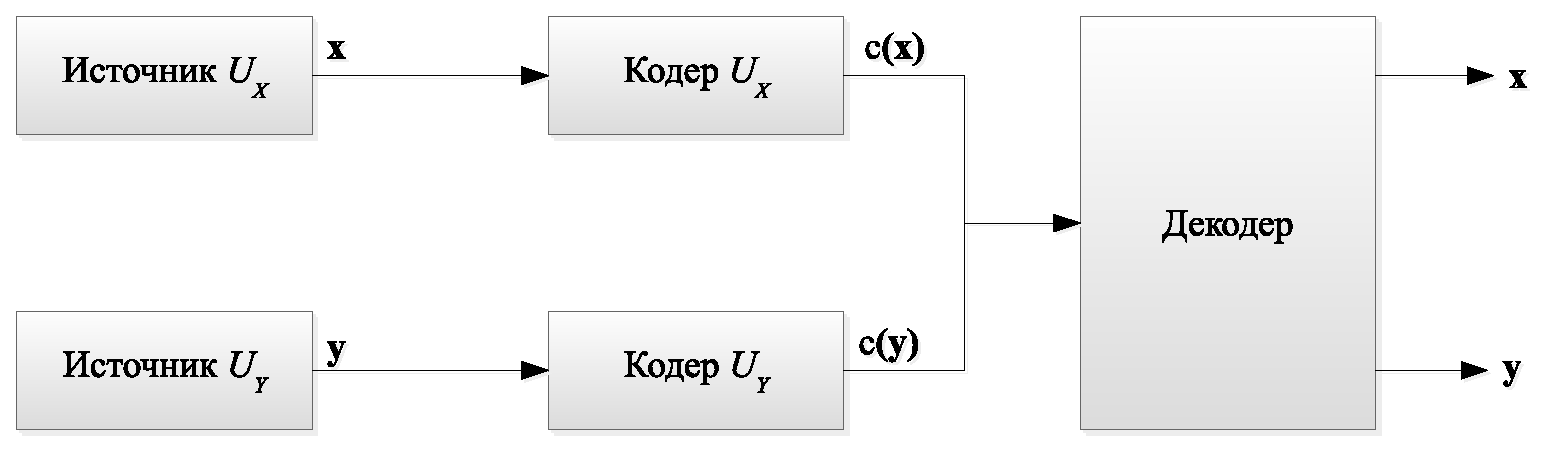
\includegraphics[width=\textwidth]{Chapter1/SWSystem}
\caption{Структура системы обработки информации с использованием независимого кодирования зависимых источников}
\label{fig:SWSystem}
\end{center}
\end{figure}

Одним из ключевых результатов работы~\cite{Slepian1973} является определение области допустимых скоростей для случая независимого кодирования и совместного декодирования источников. В такой системе обработки информации кодирование выходов каждого из источников выполняется независимо от другого своим собственным кодером. Кодер источника $U_X$ отображает последовательность символов $\mathbf{x}$ в двоичную последовательность $c(\mathbf{x})$, кодер $U_Y$ отображает $\mathbf{y}$ в $c(\mathbf{y})$. Обозначим через $H(X,Y)$, $H(X \vert Y)$, $H(Y \vert X)$  энтропии, определяемые из совместного распределения $p(\mathbf{x},\mathbf{y})$. Любая пара чисел $(r_X,r_Y)$, удовлетворяющая следующим соотношениям:
\begin{equation*}
\begin{split}
r_X & \geq H(X \vert Y) \\
r_Y & \geq H(Y \vert X) \\
r_X + r_Y & \geq H(X,Y)
\end{split},
\label{eq:SWRate}
\end{equation*}
является парой допустимых скоростей при независимом кодировании и совместном декодировании зависимых источников. Этот регион скоростей представлен графически на рисунке~\ref{fig:SWRates}. Приведенное выше утверждение известно как прямая теорема кодирования зависимых источников. Доказательство можно найти, например, в работе~\cite{Slepian1973} или в учебнике~\cite{Kolesnik}.

\begin{figure}[htbp]
\begin{center}
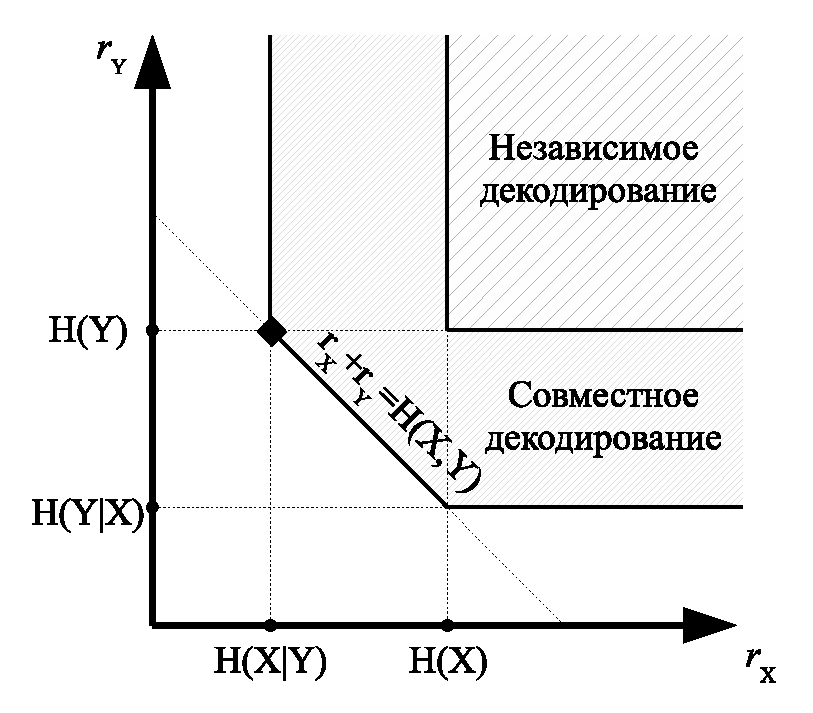
\includegraphics[width=0.5\textwidth]{Chapter1/SWRates}
\caption{Область допустимых скоростей при кодировании зависимых источников}
\label{fig:SWRates}
\end{center}
\end{figure}

Основной результат данной теоремы заключается в том, что независимое кодирование зависимых источников без памяти не приводит в общем к увеличению минимальной допустимой суммарной скорости кодирования по сравнению с совместным кодированием.

Процесс сжатия в описанной выше системе обработки информации принято называть кодированием Слепяна-Вулфа (Slepian-Wolf coding). Отметим, что кодирование Слепяна-Вулфа является сжатием без потерь, т.~к. в процессе совместного декодирования обе последовательности восстанавливаются с произвольно малой вероятностью ошибки.

В 1976 году Вайнер и Зив~\cite{Wyner1976} рассмотрели частный случай кодирования зависимых источников, когда требуется сжать с потерями выход источника $U_X$, если на декодере доступен без потерь выход $U_Y$ (рисунок~\ref{fig:WZSystem}). В таком случае, говорят, что $\mathbf{y}$~--~это дополнительная информация декодера, а процесс сжатия в такой системе называют кодированием с дополнительной информацией на декодере. В англоязычной литературе для обозначения дополнительной информации используют термин \emph{Side Information} (сторонняя информация). Графическое представление такой системы передачи информации приведено на рисунке~\ref{fig:WZSystem}. Вайнер и Зив исследовали поведение функции <<скорость-искажение>>~\cite{kudryashow2009} и показали, что в общем случае эффективность сжатия в такой системе ниже, чем в схеме с совместным кодированием. Однако, в некоторых случаях, в частности, когда источники $U_X$ и $U_Y$ являются совместно Гауссовыми, а в качестве меры потерь используется функция среднеквадратичной ошибки, кривые <<скорость-искажение>> совпадают. Этот результат известен как теорема Вайнера-Зива, доказательство которой можно найти в работе~\cite{Wyner1976}.

\begin{figure}[htbp]
\begin{center}
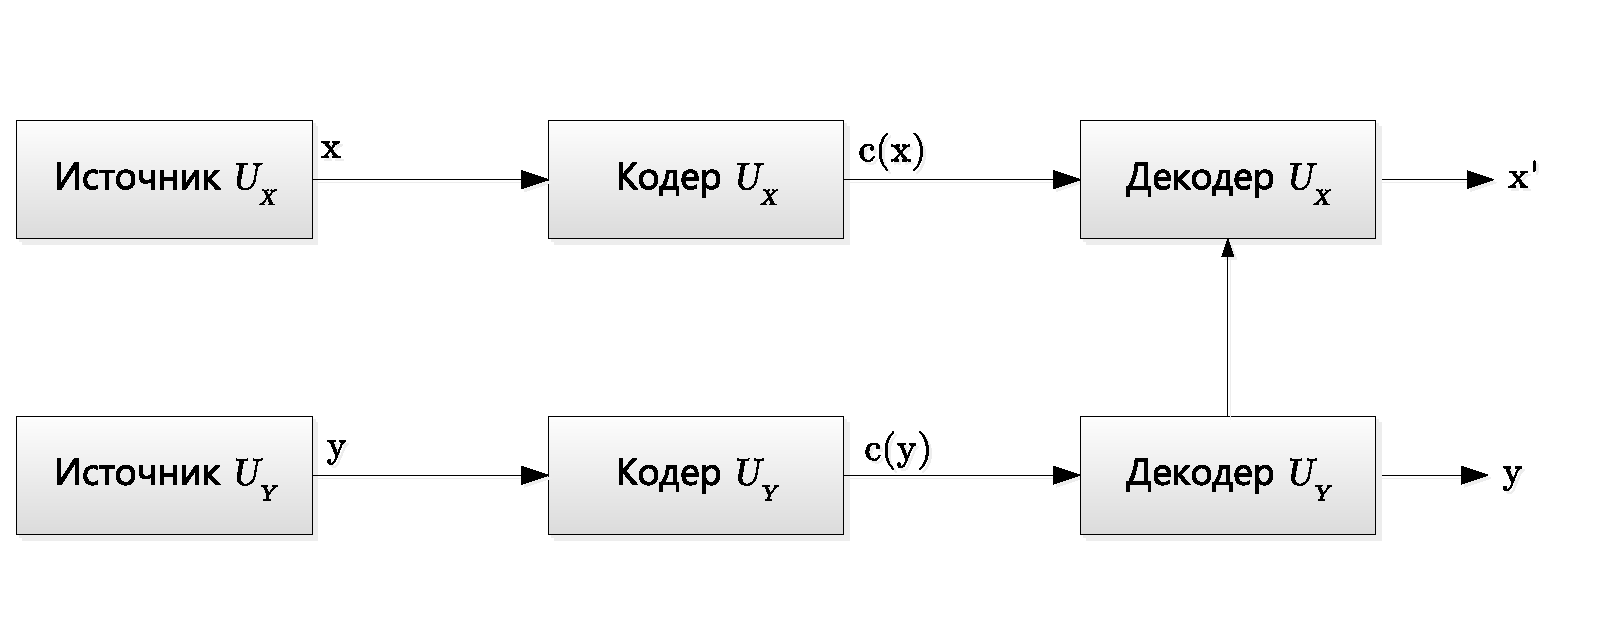
\includegraphics[width=\textwidth]{Chapter1/WZSystem}
\caption{Структура системы передачи информации при кодировании зависимых источников с дополнительной информацией на декодере}
\label{fig:WZSystem}
\end{center}
\end{figure}

Теоретические результаты, приведенные в работах Слепяна-Вулфа и Вайнера-Зива, предполагают, что возможно сжать выходы двух зависимых источников с использованием методов распределенного кодирования (независимое кодирование и совместное декодирование), при этом не потеряв в эффективности сжатия по сравнению со схемами, основанными на совместном кодировании и декодировании. В работе~\cite{Pradhan2003} утверждается, например, что система с кодированием при наличии дополнительной информации на декодере не проигрывает совместному кодированию, в том случае, если разница между выходами источников является Гауссовой.

\section{Применение помехоустойчивого кодирования для сжатия информации}\label{chap1:2}
Практические подходы к распределенному кодированию зависимых источников во многом связаны с методами помехоустойчивого кодирования. В связи с этим перед описанием применения распределенного кодирования для сжатия видеоданных рассмотрим несколько простых примеров, показывающих реализацию распределенного кодирования на практике с использованием методов помехоустойчивого кодирования.

Так как символы на выходе источников $U_X$ и $U_Y$ обладают взаимной корреляцией, то вектор $\mathbf{y}$ можно рассматривать как искаженную версию вектора $\mathbf{x}$. В таком случае, процесс обработки данных в распределенном кодировании можно интерпретировать следующим образом (рисунок~\ref{fig:ChannelCodeAnalogue}). Последовательность $\mathbf{x}$ передается через некоторый канал с шумом. В результате на декодер поступает новая последовательность $\mathbf{y}$, причем
\begin{equation*}
\mathbf{y} = \mathbf{x} + \mathbf{n},
\end{equation*}
где вектор $\mathbf{n}$ описывает шум (различия между $\mathbf{y}$ и $\mathbf{x}$).

\begin{figure}[htbp]
\begin{center}
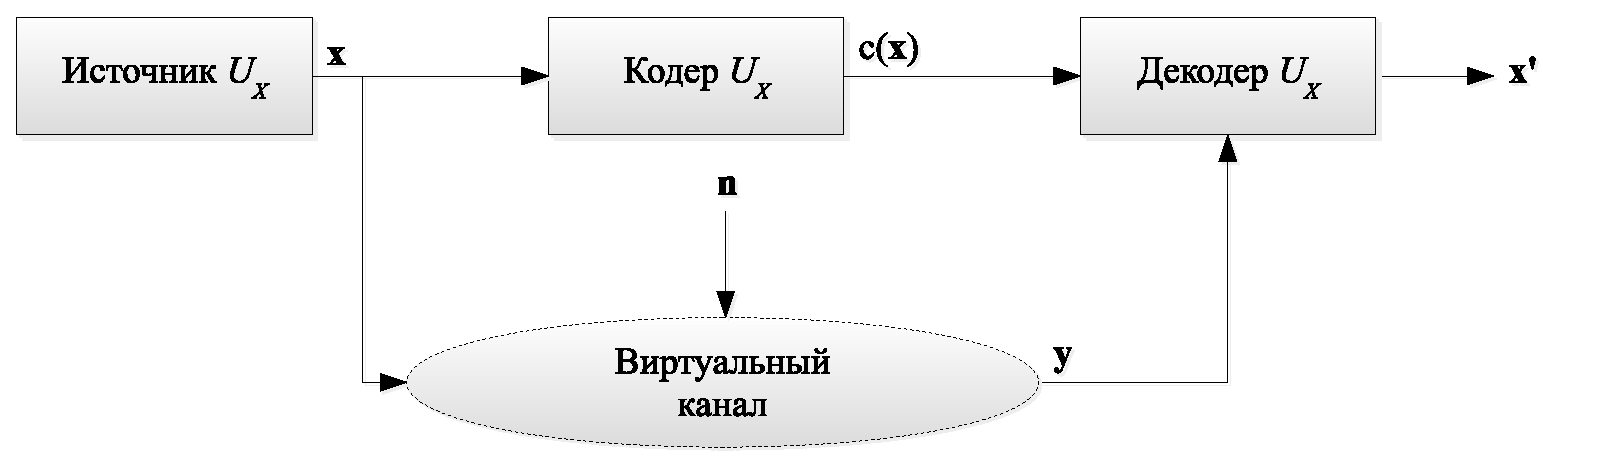
\includegraphics[width=\textwidth]{Chapter1/ChannelCodeAnalogue}
\caption{Альтернативная интерпретация кодирования с дополнительной информацией на декодере}
\label{fig:ChannelCodeAnalogue}
\end{center}
\end{figure}

Задача совместного декодера сводится к тому, чтобы устранить шумовые составляющие из $\mathbf{y}$ и восстановить $\mathbf{x}$, т.~е. исправить ошибки, <<возникшие>> в процессе передачи по каналу. В распределенном кодировании принято называть описанный выше канал \textit{каналом с виртуальной зависимостью} или \textit{виртуальным каналом}, а <<возникающий>> в нем шум~--~ \textit{корреляционным шумом} (Correlation Noise). Задача кодера источника $U_X$ в таком случае заключается в том, чтобы выполнить помехоустойчивое кодирование последовательности $\mathbf{x}$ и отослать совместному декодеру проверочную информацию. При этом считается, что проверочная информация передается без ошибок. Сжатие достигается в том случае, если средний объем проверочной информации, достаточной для восстановления исходной последовательности $\mathbf{x}$, меньше объема исходной последовательности.

В качестве демонстрации применения методов помехоустойчивого кодирования в задаче сжатия зависимых источников, а также для того, чтобы представить  реализацию схемы кодирования Слепяна-Вулфа на практике, рассмотрим следующий пример~\cite{1184140}. Пусть на выходе источников $U_X$ и $U_Y$ наблюдаются равновероятные последовательности $\mathbf{x}_i \in \mathcal{X}$ и $\mathbf{y}_i \in \mathcal{Y}$ двоичных символов длины $m=3$, т.~е. $\mathcal{X}=\mathcal{Y}=\{0,1\}^3$. Будем считать, что выходы источников являются зависимыми, причем зависимость выражается в том, что расстояние Хэмминга между каждой парой $\mathbf{x}_i$ и $\mathbf{y}_i$ не превышает единицу, т. е. последовательности различаются не более, чем в одной позиции.  В качестве примера рассмотрим передачу сообщений, состоящих из одного символа ($n=1$): $\mathbf{x}_1=(101)$, $\mathbf{y}_1=(100)$. Для упрощения обозначений далее не будем указывать индекс $1$. Рассмотрим три схемы кодирования и определим для каждой из них минимальную скорость (минимальное число бит, которое кодер должен передать декодеру), необходимую для точного восстановления выходов обоих источников на декодере.

\begin{enumerate}
\item \emph{Независимое кодирование и декодирование} (рисунок~\ref{fig:Example1a}).
Выходы источников $U_X$ и $U_Y$ кодируются и декодируются независимо друг от друга. В таком случае, так как последовательности на выходе источников являются равновероятными, суммарную минимальную скорость можно определить следующим образом:
\begin{equation*}
\begin{split}
& r_{XY}^{(1)} = r_X + r_Y = \\
& - \sum\limits_{ \mathbf{x} \in \{0,1\}^3} p(\mathbf{x}) \log_2(p(\mathbf{x})) - 
\sum\limits_{ \mathbf{y} \in \{0,1\}^3} p(\mathbf{y}) \log_2(p(\mathbf{y})) = \\
& = - \sum\limits_{ \mathbf{x} \in \{0,1\}^3} \frac{1}{8} \log_2\frac{1}{8} - 
\sum\limits_{ \mathbf{y} \in \{0,1\}^3} \frac{1}{8} \log_2\frac{1}{8} = 3 + 3 = 6 \text{ бит}
\end{split}.
\end{equation*}

\begin{figure}[thbp]
\begin{center}
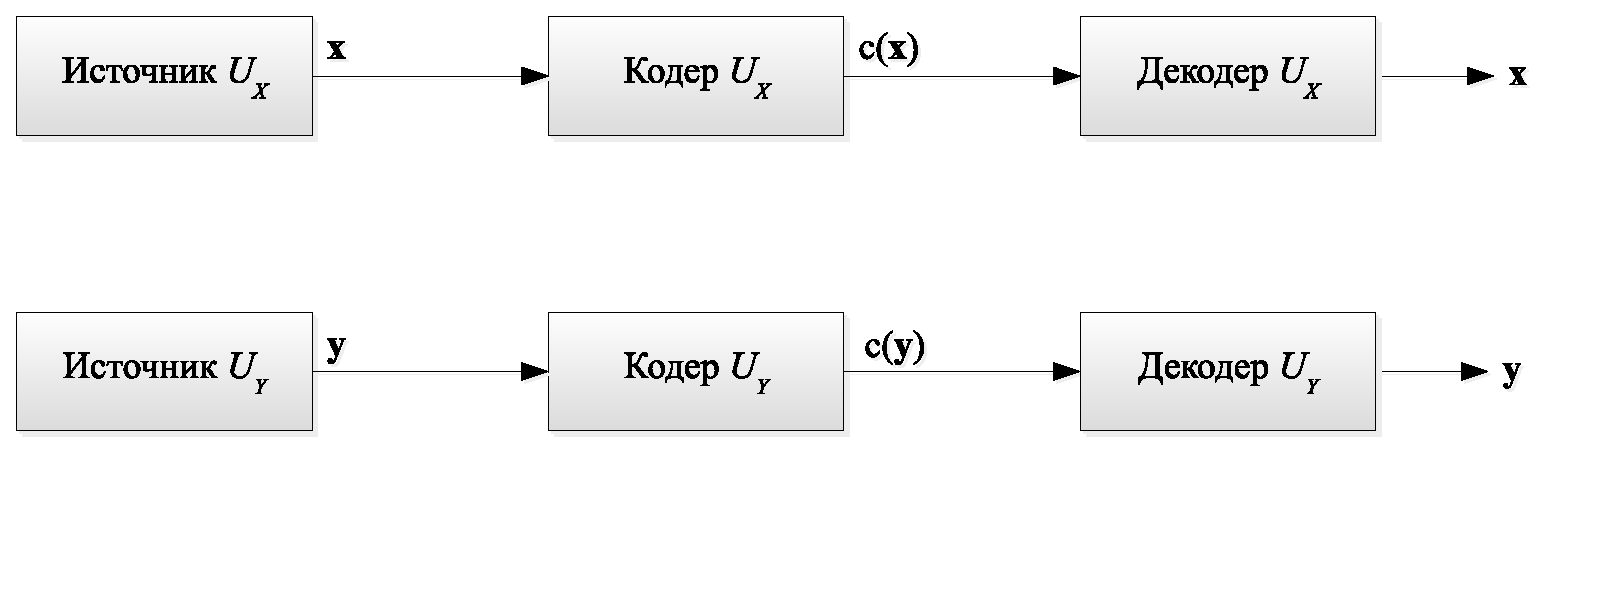
\includegraphics[width=0.9\textwidth]{Chapter1/Example1a}
\caption{Система передачи информации с независимой обработкой}
\label{fig:Example1a}
\end{center}
\end{figure}

Таким образом, при независимом кодировании источников $U_X$ и $U_Y$ необходимо передать 6 бит, для того, чтобы декодер смог восстановить последовательности без потерь. Для данного примера кодер должен отправить декодеру вектор $\mathbf{v}^{(1)}=(101100)$, который получается простой конкатенацией векторов $\mathbf{x}$ и $\mathbf{y}$.

\item \emph{Совместное кодирование и декодирование} (рисунок~\ref{fig:Example1b}).

Выходы источников кодируются совместно, декодирование тоже происходит совместно. Так как расстояние Хэмминга между $\mathbf{x}$ и $\mathbf{y}$ не превышает единицу, вектор-разница $\mathbf{z}$ между этими последовательности принадлежит упорядоченному множеству $\mathcal{Z}=\{000, 001, 010, 100\}$, причем элементы этого множества равновероятны. Если последовательность $\mathbf{y}$ известна и кодеру, и декодеру, то для передачи $\mathbf{x}$ достаточно закодировать только индекс вектора-разницы. Минимальная суммарная скорость в такой системе определяется как:
\begin{equation*}
\begin{split}
& r_{XY}^{(2)} = r_{\mathcal{Z}} + r_Y = \\
& - \sum\limits_{ \mathbf{z} \in \mathcal{Z}} p(\mathbf{z}) \log_2(p(\mathbf{z})) - 
\sum\limits_{ \mathbf{y} \in \{0,1\}^3} p(\mathbf{y}) \log_2(p(\mathbf{y})) = \\
& = - \sum\limits_{ \mathbf{z} \in Z} \frac{1}{4} \log_2\frac{1}{4} - 
\sum\limits_{ \mathbf{y} \in \{0,1\}^3} \frac{1}{8} \log_2\frac{1}{8} = 2 + 3 = 5 \text{ бит}.
\end{split}
\end{equation*}

\begin{figure}[thbp]
\begin{center}
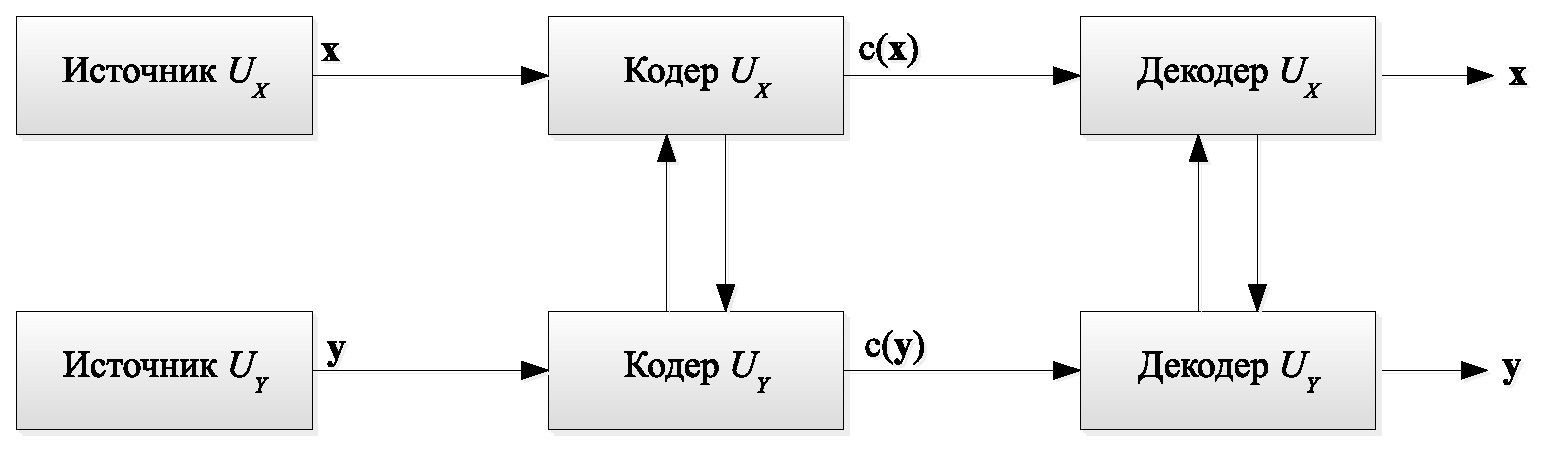
\includegraphics[width=0.9\textwidth]{Chapter1/Example1b}
\caption{Система передачи информации с совместной обработкой}
\label{fig:Example1b}
\end{center}
\end{figure}

Таким образом, при совместном кодировании источников $U_X$ и $U_Y$ декодеру необходимо передать 5 бит, для того, чтобы он смог восстановить последовательности без потерь. При этом считается, что множество $\mathcal{Z}$ известно кодеру и декодеру.

В данном примере кодер должен отправить вектор $\mathbf{v}^{(2)}=(10001)$, в котором первые три бита $ (100) $ представляют собой последовательность $\mathbf{y}$, а последние два бита $(01)$ являются двоичным представлением  индекса вектора в множестве $\mathcal{Z}$, который в данном примере равен
\begin{equation*}
\mathbf{z} = \mathbf{x} + \mathbf{y} = (101) + (100) = (001).
\end{equation*}

Декодер, получив последовательность $\mathbf{v}^{(2)}$, выделяет из неё сообщение $\mathbf{y}$ и индекс элемента в $\mathcal{Z}$. Далее соответствующий элемент $\mathcal{Z}$ складывается с $\mathbf{y}$ для того, чтобы получить $\mathbf{x}$:
\begin{equation*}
\mathbf{y} + \mathcal{Z}(1) = (100) + (001) = (101) = \mathbf{x}.
\end{equation*}

Таким образом, декодер безошибочно восстанавливает оба сообщения.

\item \emph{Независимое кодирование и совместное декодирование} (рисунок~\ref{fig:Example1c}).

В такой системе кодирование выходов источников осуществляется независимо, декодер сначала восстанавливает последовательность $\mathbf{y}$ и, зная $\mathbf{y}$, восстанавливает $\mathbf{x}$. Определим, сколько бит должен передать кодер декодеру, чтобы тот смог точно восстановить $\mathbf{x}$. 

\begin{figure}[thbp]
\begin{center}
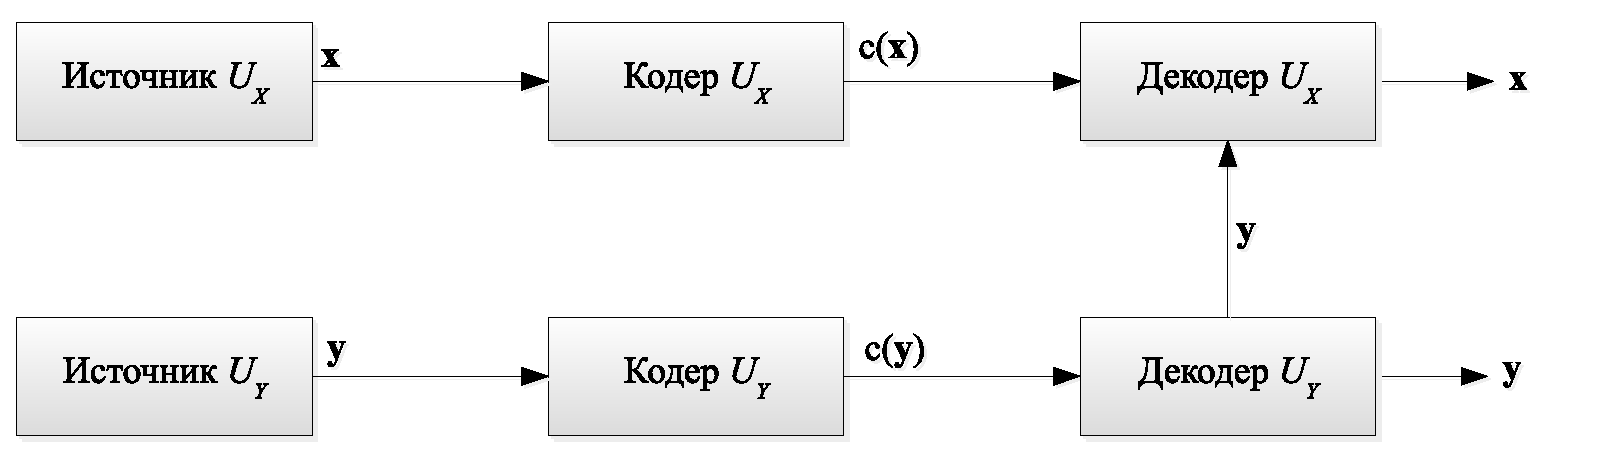
\includegraphics[width=0.9\textwidth]{Chapter1/Example1c}
\caption{Система передачи с обработкой информации по схеме Вайнера-Зива}
\label{fig:Example1c}
\end{center}
\end{figure}

Введем в рассмотрение следующую проверочную матрицу линейного кода:
\begin{equation*}
\mathbf{H} = \begin{pmatrix} 
    1 & 1 & 0 \\
    1 & 0 & 1
\end{pmatrix}.
\end{equation*}

Будем считать, что эта матрица известна кодеру и декодеру. Кодер рассчитывает синдром последовательности $\mathbf{x}$:
\begin{equation*}
\mathbf{s} = \mathbf{x}^T\mathbf{H}^T,
\end{equation*}
где $\mathbf{s} \in \mathcal{S}$ и $\mathcal{Z} = \{0,1\}^2$~--~множество всех возможных синдромов для рассмотренного линейного кода.

Далее синдром $\mathbf{s}$ пересылается декодеру, который определяет смежный класс для вектора полученного синдрома $\mathbf{s}$ по таблице стандартной расстановки линейного кода, которая известна для матрицы $\mathbf{H}$ и строится на декодере заранее. Декодер находит лидера смежного класса, как вектор, ближайший по расстоянию Хэмминга к уже восстановленному вектору $\mathbf{y}$. Лидер смежного класса и есть восстановленный вектор $\mathbf{x}$. Определим минимальное количество бит, необходимых для точного восстановления обеих последовательностей:
\begin{equation*}
\begin{split}
& r_{XY}^{(3)} = r_S + r_Y = \\
& - \sum\limits_{ \mathbf{s} \in S} p(\mathbf{s}) \log_2(p(\mathbf{s})) - 
\sum\limits_{ \mathbf{y} \in \{0,1\}^3} p(\mathbf{y}) \log_2(p(\mathbf{y})) = \\
& = - \sum\limits_{ \mathbf{s} \in S} \frac{1}{4} \log_2\frac{1}{4} - 
\sum\limits_{ \mathbf{y} \in \{0,1\}^3} \frac{1}{8} \log_2\frac{1}{8} = 2 + 3 = 5 \text{ бит}
\end{split}.
\end{equation*}

В рассматриваемом примере синдром последовательности $\mathbf{x}$, рассчитанный кодером:

\begin{equation*}
\mathbf{s} = \mathbf{x}^T\mathbf{H}^T = (101) \begin{pmatrix} 1 & 1 \\ 1 & 0 \\ 0 & 1 \end{pmatrix} = (10)
\end{equation*}

Биты синдрома передаются декодеру. Таблица стандартной расстановки для рассматриваемого кода представлена в таблице~\ref{tab:Cosets}.
\begin{table}[!h]
    \caption{Таблица стандартной расстановки}
    \begin{center}
        \label{tab:Cosets}
        \begin{tabular}{|c|c|}
            \hline
            Синдром & Смежный класс \\
            \hline
            (00) & \{(000),(111)\} \\ 
            \hline
            (01) & \{(001),(011)\} \\ 
            \hline
            (10) & \{(010),(101)\} \\ 
            \hline
            (11) & \{(100),(011)\} \\ 
            \hline
        \end{tabular}
    \end{center}
\end{table}
%\begin{equation*}
%\begin{array}{|c|c|}
%\hline
%\text{Синдром} & \text{Смежный класс} \\ \hline
%(00) & \{(000),(111)\} \\ \hline
%(01) & \{(001),(011)\} \\ \hline
%(10) & \{(010),(101)\} \\ \hline
%(11) & \{(100),(011)\} \\ \hline
%\end{array}
%\end{equation*}

Смежный класс для полученного синдрома $\{(010),(101)\}$. Найдем лидера смежного класса, зная, что $\mathbf{y}=(100)$. Найдем расстояние Хэмминга между $\mathbf{y}=(100)$ и векторами из смежного класса:
\begin{equation*}
\begin{split}
& (100) + (010) = 2 \\
& (100) + (101) = 1
\end{split}.
\end{equation*}

Таким образом, лидер смежного класса~--~это вектор $(101)$. Отметим, что этот вектор совпадает с последовательностью $\mathbf{x}$, т.~е. удалось успешно выполнить декодирование. При этом кодер отправил декодеру $5$ бит, что совпадает со скоростью, полученной в случае совместных кодирования и декодирования, т. е. $r_{XY}^{(3)}=r_{XY}^{(2)} < r_{XY}^{(1)}$.

\end{enumerate}

Приведенные выше примеры являются демонстрацией практического применения методов распределенного кодирования для сжатия двух простых зависимых источников, на выходе которых наблюдаются одномерные векторы с коррелированными символами. Однако отметим, что видеопоследовательности представляют собой многомерные (например, два измерения на представление одной сцены и третье измерение на представление изменений в сцене во времени) данные, в связи с чем далее рассмотрим примение распределенного кодирования для сжатия видеоданных.

\section{Пример реализации распределенного кодирования видеоисточников в рамках простой модели видеопотока}
\label{chap1:3}

В начале 2000-х годов на основании теорем Вайнера-Зива и Слепяна-Вулфа был сформирован новый подход к сжатию видеоданных, известный как \emph{распределенное кодирование видеоданных} (Distributed Video Coding, DVC, или Wyner-Ziv Video Coding, WZVC)~\cite{1197184}. В этом подходе сжимаемая видеопоследовательность интерпретируется как выход от нескольких зависимых источников, при этом источники могут порождать как кадры целиком, так и части кадров. Наиболее распространенной схемой является схема с двумя источниками, которые обрабатываются по следующим правилам:
\begin{itemize}
\item выход первого источника обрабатывается в независимом режиме (по аналогии с источником $U_Y$, рассмотренным ранее);
\item выход второго источника кодируется независимо, но декодирование осуществляется с учетом восстановленных данных первого источника (по аналогии с источником $U_X$, рассмотренным ранее).
\end{itemize}

Перед тем, как рассматривать практические реализации распределенных кодеков видеоданных, приведем ещё один пример. Данный пример не демонстрирует новых принципов сжатия, однако позволяет получить некоторые оценки на простой модели видеоданных, как последовательности двумерных данных (кадров), имеющих зависимость во времени, а также улучшить качественное понимание системы в целом.

Рассмотрим видеопоследовательность, состоящую из трех черно-белых кадров размером $5$ пикселей в высоту и $5$ пикселей в ширину. Единственным движущимся объектом на кадрах является черная точка (один пиксель) на белом фоне, начальное положение точки фиксировано и находится в центре кадра. Между соседними кадрами точка должна изменить свое местоположение, перейдя в один из 8 соседних пикселей (рисунок~\ref{fig:Example2a}). Будем считать, что вероятности переходов равны.
\begin{figure}[htbp]
\begin{center}
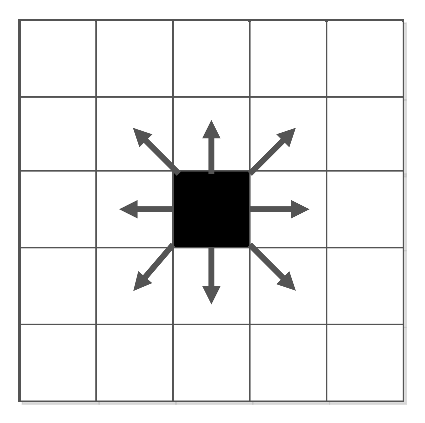
\includegraphics[width=0.3\textwidth]{Chapter1/Example2a}
\caption{Возможные направления смещения точки между соседними кадрами}
\label{fig:Example2a}
\end{center}
\end{figure}

Для того, чтобы сжать такую видеопоследовательность достаточно передать информацию о траектории движения точки. Рассмотрим два возможных сценария кодирования информации о траектории. Обобщенная схема системы передачи для обоих сценариев приведена на рисунке~\ref{fig:Example2b}. Данная система включает два источника информации $U_Y$ и $U_X$. Будем считать, что видеопоследовательность была заранее разбита на две подпоследовательности таким образом, что на выходе источника $U_Y$ появляются кадры с номерами $1$ и $3$, а на выходе источника $U_X$~–~кадр $2$.

Также в системе передачи информации присутствует ключ, определяющий режим работы кодеров источников. Если ключ разомкнут ($K=0$), кодеры не взаимодействуют друг с другом, т.~е. этот сценарий соответствует случаю независимого кодирования и совместного декодирования выходов зависимых источников $U_Y$ и $U_X$. Если ключ замкнут ($K=1$), то сжатие информации, поступающей от источников, выполняется совместно, т.~е. этот сценарий соответствует совместному кодированию и декодированию.

\begin{figure}[htbp]
\begin{center}
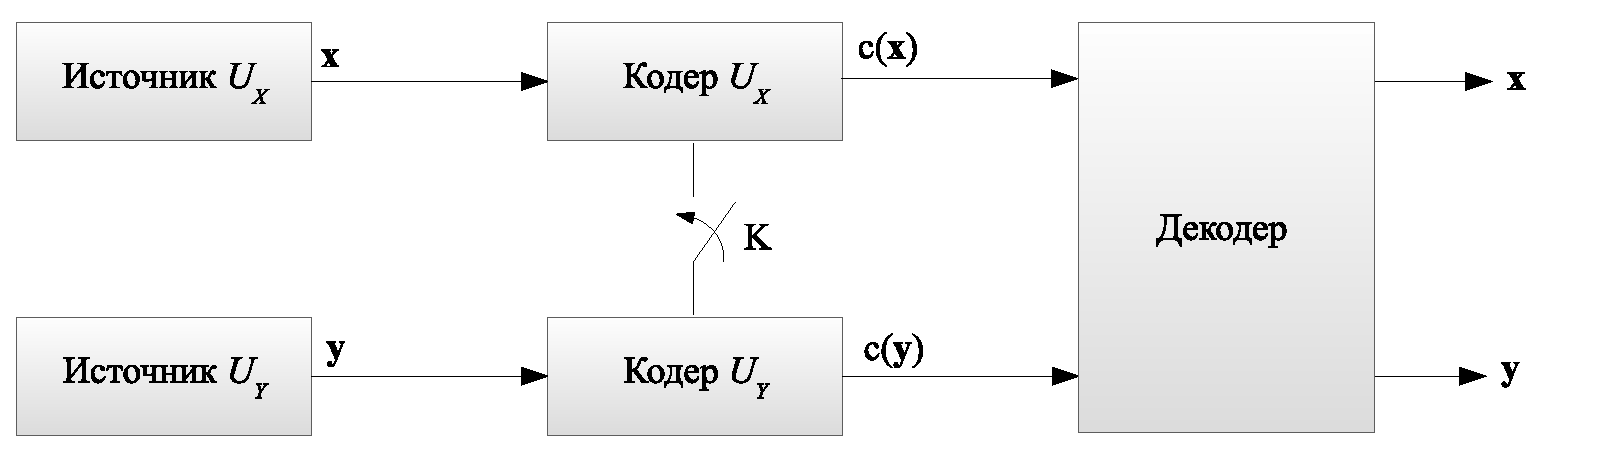
\includegraphics[width=\textwidth]{Chapter1/Example2b}
\caption{Структурная схема обобщенной системы передачи информации от зависимых источников с общим декодером}
\label{fig:Example2b}
\end{center}
\end{figure}

\begin{enumerate}

\item Определим сколько бит нужно для кодирования всех кадров, когда ключ $K$ замкнут. Пусть величина $r_{2 \vert 1}$ показывает сколько бит необходимо передать декодеру, чтобы он смог восстановить положение черной точки на втором кадре. Т.к. есть 8 возможных равновероятных сдвигов, то число бит, которое необходимо затратить в таком случае равно $\log_{2}8=3$ бита. Аналогичные рассуждения позволяют рассчитать значение $r_{3 \vert 2}$. В результате:
\begin{equation*}
r_{K=0} = r_1 + r_{2 \vert 1} + r_{3 \vert 2} = 0 + \log_28 + \log_28 = 6\text{ бит}.
\end{equation*}

\item Определим сколько бит нужно для кодирования всех кадров, когда ключ $K$ разомкнут. Опишем возможный способ сжатия видеопоследовательности в такой системе передачи информации.

\begin{enumerate}
\item Кодер источника $U_Y$ передает сжатую информацию о кадрах $1$ и $3$ совместному декодеру.
\item Декодер по обратной связи передает кодеру $U_X$ информацию о положении черного пикселя в кадре $3$.
\item Кодер источника $U_X$ отправляет совместному декодеру некоторое количество вспомогательных бит, которые позволяют ему восстановить координаты черного пикселя на кадре $2$.
\end{enumerate}
Найдем среднее число бит для такого способа сжатия:
\begin{equation*}
r_{K=1}^{(1)} = r_Y + r_X,
\end{equation*}
где $r_Y$ - битовые затраты на передачу информации о положении точки в кадрах $1$ и $3$, $r_X$ - битовые затраты на передачу информации о положении точки в кадре $2$.
\begin{equation*}
r_Y = r_1 + r_{3 \vert 1},
\end{equation*}
где $r_{3 \vert 1}$ - количество бит, необходимых для передачи информации о положении пикселя в кадре 3 при известном кадре 1. Вероятности появления пикселя в определенных позициях кадра 3 приведены в следующей матрице:
\begin{equation*}
\mathbf{P}_{3 \vert 1} = \frac{1}{64}
\begin{pmatrix}
1 & 2 & 3 & 2 & 1 \\
2 & 2 & 4 & 2 & 2 \\
3 & 4 & 8 & 4 & 3 \\
2 & 2 & 4 & 2 & 2 \\
1 & 2 & 3 & 2 & 1
\end{pmatrix}.
\end{equation*}
Таким образом,
\begin{equation*}
r_Y = 0 + \sum\limits_{i=1}^{5}\sum\limits_{j=1}^{5}\mathbf{P}_{3 \vert 1}[i,j]\log_2 \mathbf{P}_{3 \vert 1}[i,j] = 4.4528\text{ бит}.
\end{equation*}
Определим теперь среднее число бит, которые кодер источника $U_X$ должен отправить совместному декодеру, зная положение черного пикселя в кадре $3$. Это число определяется координатами пикселя в кадре $3$ и количеством траекторий, ведущих из центра (положения пикселя в кадре $0$) в эти координаты. Количество возможных траекторий приведено в матрице $\mathbf{L}$:
\begin{equation*}
\mathbf{L} =
\begin{pmatrix}
1 & 2 & 3 & 2 & 1 \\
2 & 2 & 4 & 2 & 2 \\
3 & 4 & 8 & 4 & 3 \\
2 & 2 & 4 & 2 & 2 \\
1 & 2 & 3 & 2 & 1
\end{pmatrix}.
\end{equation*}

Среднее число бит для последнего шага можно найти по следующей формуле:

\begin{equation*}
r_X = \sum\limits_{i=1}^{5}\sum\limits_{j=1}^{5} \mathbf{P}_{3 \vert 1}[i,j]\log_2 \mathbf{L}[i,j] = 1.5472\text{ бит}.
\end{equation*}

В таком случае среднее число бит, затрачиваемых на сжатие всей последовательности:
\begin{equation*}
r_{K=1}^{(1)} = r_Y + r_X = 4.4528 + 1.5472 = 6\text{ бит.}
\end{equation*}

Рассмотрим альтернативный способ сжатия видеопоследовательности.

\begin{enumerate}
\item\label{it:ex2:2:a} Кодер источника $U_Y$ передает сжатую информацию о кадрах $1$ и $3$ совместному декодеру.
\item\label{it:ex2:2:b} Кодер источника $U_X$ передает декодеру контрольную информацию, например CRC~\cite{Koopman04cyclicredundancy}, рассчитанную для кадра $2$.
\item\label{it:ex2:2:c} Декодер строит некоторую оценку положения черной точки в кадре $2$, считает контрольную информацию по этой оценке и сравнивает с данными, полученными от кодера. Если контрольная информация совпадает, то декодер считает, что ему удалось декодировать кадр $2$. В противном случае декодер запрашивает дополнительную информацию у кодера.
\item\label{it:ex2:2:d} При наличии запроса от декодера кодер источника $U_X$ отправляет декодеру некоторое количество вспомогательных бит, которые позволяют ему восстановить промежуточное положение черного пикселя на кадре $2$.
\end{enumerate}

Определим среднее количество бит, которые нужно передать для этой процедуры, без учета контрольной информации.

Шаг~a) совпадает с тем же шагом описанного ранее алгоритма и требует $4.4528$ бит. Шаг~d) схож с шагом~с) предыдущего алгоритма, за исключением того, что нужно учесть то, что декодер может иногда угадать положение точки в кадре $2$. Таким образом, формула для расчета среднего числа бит для шага~d) выглядит следующим образом:
\begin{equation*}
r_d = \sum\limits_{i=1}^{5}\sum\limits_{j=1}^{5} \mathbf{P}_{3 \vert 1}[i,j]p_f(i,j)\log_2 \mathbf{L}[i,j],
\end{equation*}
где через $p_f(i,j)$ обозначена вероятность события, что декодер не угадал положение точки в кадре $2$, при условии того, что в кадре $3$ точка находится в клетке с координатами $(i,j)$:
\begin{equation*}
p_f(i,j) = \frac{\mathbf{L}[i,j]-1}{\mathbf{L}[i,j]}.
\end{equation*}

В результате:
\begin{equation*}
r_d = \sum\limits_{i=1}^{5}\sum\limits_{j=1}^{5}\mathbf{P}_{3 \vert 1}[i,j]\frac{\mathbf{L}[i,j]-1}{\mathbf{L}[i,j]}\log_2 \mathbf{L}[i,j] = 1.0884\text{ бит}.
\end{equation*}

Для рассмотренного алгоритма можно сделать два вывода.
\begin{enumerate}
\item Если для передачи CRC в среднем использовать $0.4558$ бит, то описанная процедура не будет проигрывать кодированию с учетом зависимости между кадрами.
\item С вероятностью $p_s$ декодер может угадать положение черного пикселя на кадре 1:
\begin{equation*}
p_s = \sum\limits_{i=1}^{5}\sum\limits_{j=1}^{5} \mathbf{P}_{3 \vert 1}[i,j]\left(1-\frac{\mathbf{L}[i,j]-1}{\mathbf{L}[i,j]}\right) = 0.3906.
\end{equation*}

\end{enumerate}

\end{enumerate}

Рассмотрим теперь существующие кодеки, основанные на принципах кодирования зависимых источников.

\section{Классификация методов распределенного кодирования источников видеоинформации}
\label{chap:DVC:Classification}

Для удобства дальнейшего изложения введем в рассмотрение классификацию методов распределенного кодирования (рисунок~\ref{fig:Classification}). Данная классификация будет использоваться при описании основных концепций распределенного видеокодирования. Методы распределенного кодирования источников видеоинформации в зависимости от ряда признаков можно классифицировать следующим образом.

\begin{itemize}
    \item По типу обрабатываемых данных.
    \begin{itemize}
        \item \emph{Обработка кадров целиком}. В методах распределенного кодирования, основанных на обработке кадров целиком, выходами зависимых источников считаются кадры видеопоследовательности. Такой подход является обоснованным с точки зрения теории кодирования зависимых источников в силу того, что близкие во времени кадры как правило обладают высокой временной зависимостью. Таким образом, в первую очередь осуществляется устранение временной избыточности.
        \item \emph{Обработка частей кадров}. Распределенное кодирование в подобных методах используется для устранения как межкадровой, так и внутрикадровой избыточности. Кадры разбиваются на непересекающиеся блоки, и для каждого блока принимается решение о принадлежности к одному из зависимых источников. Тип кодирования определяется в зависимости от принятого решения.
    \end{itemize}
    \item По наличию обратной связи от декодера к кодеру.
    \begin{itemize}
        \item \emph{С обратной связью}. В подобных методах между кодером и декодером есть обратная связь, по которой декодер может запрашивать некоторую вспомогательную информацию, например, с целью управления битовой скоростью.
        \item \emph{Без обратной связи}. В методах данного класса декодер не может запрашивать у кодера дополнительную информацию. Следует отметить, что в таком случае, если декодеру не удается успешно декодировать данные зависимого источника, сжатие возможно только с потерями.
    \end{itemize}
    \item По области обработки.
    \begin{itemize}
        \item \emph{Обработка в пространстве пикселей} (в пиксельном домене). В подобных методах считается, что зависимые источники порождают непосредственно пиксели изображений. Схемы, основанные на сжатии в пространстве пикселей, характеризуются, как правило, очень низкой вычислительной сложностью на стороне кодера, т.~к. сжатию подвергаются непосредственно значения интенсивностей цветовых компонент кадров. Существенным недостатком подобных подходов является низкая гибкость, заключающаяся в невозможности эффективно выделять и устранять пространственную избыточность, присущую кадрам видео.
        \item \emph{Обработка в преобразованном пространстве} (в преобразованном домене). В методах, принадлежащих данному классу, считается, что зависимые источники порождают сообщения, которые представляют собой некоторые функции от пикселей кадров. Наиболее распространенным подходом является обработка спектральных коэффициентов, рассчитанных с использованием дискретного косинусного преобразования. Подобный подход позволяет ранжировать (классифицировать) выходы зависимых источников по степени важности с точки зрения визуального восприятия. Каждый подкласс далее может кодироваться независимо, что позволяет осуществлять эффективное управление битовой скоростью за счет масштабирования сжатого потока. 
    \end{itemize}
\end{itemize}

\begin{figure}[htbp]
    \begin{center}
        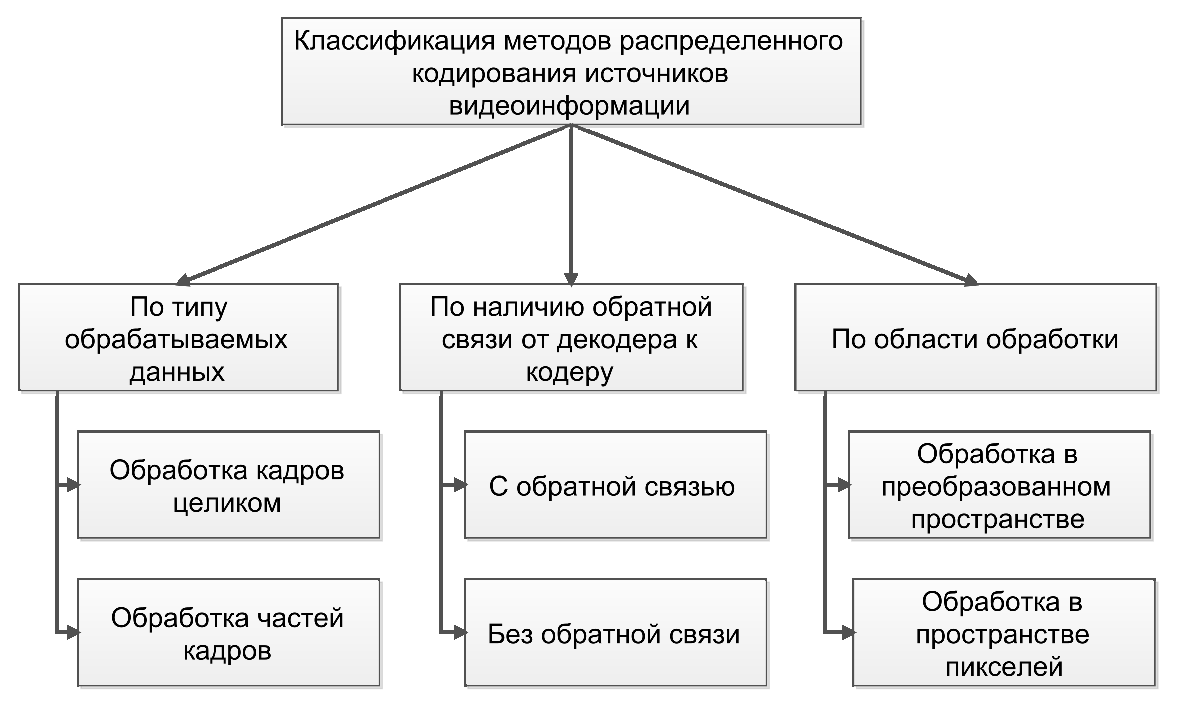
\includegraphics[width=0.8\textwidth]{Chapter1/Classification}
        \caption{Классификация методов распределенного кодирования видеоданных}
        \label{fig:Classification}
    \end{center}
\end{figure}

\section{Основные концепции распределенного кодирования источников видеоинформации}
\label{chap1:4}

\subsection{Концепция Стэнфорд}
\label{chap:DVC:Arhcs:Stan}

Концепция Стэнфорд была предложена в 2002 году для сжатия кадров в пиксельном домене~\cite{Aaron2002}, а затем была расширена для обработки спектральных коэффициентов~\cite{Aaron2004}. В основе сжатия в схеме Стэнфорд лежит использование корреляции смежных кадров видеопоследовательности. С точки зрения классификации, приведенной в подразделе~\ref{chap:DVC:Classification}, данная концепция представляет собой метод сжатия кадров в преобразованном пространстве с использованием обратной связи. Схема распределенного кодека Стэнфорд приведена на рисунке~\ref{fig:ArchStan}. Приведем на качественном уровне описание работы кодека.

\begin{figure}[htbp]
\begin{center}

\includegraphics[width=0.9\textwidth]{Chapter1/ArchStan}
\caption{Типовая схема кодека, основанного на концепции Стэнфорд}
\label{fig:ArchStan}
\end{center}
\end{figure}

\textbf{Кодер.} Видеопоследовательность разбивается на промежуточные и базовые (ключевые) кадры в блоке классификации. Промежуточные кадры будем называть \textit{ВЗ кадрами} (от Вайнер-Зив). Базовые кадры расположены в видеопоследовательности с некоторым интервалом, определяемым размером группы кадров (GOP, Group of Pictures). Ключевые кадры кодируются независимо, т.~е. без устранения временной избыточности. Такой режим обработки будем называть режимом Intra.

К ВЗ кадрам применяется блоковое спектральное преобразование, обычно дискретное косинусное преобразование. Спектральные коэффициенты со всего кадра затем группируются по следующему правилу: коэффициенты, находящиеся в разных блоках на одной и той же позиции попадают в одну группу.

Затем спектральные коэффициенты в каждой группе подвергаются равномерному квантованию, причем шаг квантования устанавливается таким, чтобы удовлетворять требуемому качеству (битовую скорость и качество восстановленного кадра с точки зрения критерия PSNR) сжатия. Квантованные спектральные коэффициенты в каждой группе далее разбиваются на битовые плоскости, которые независимо кодируются с использованием турбо кода. Кодирование начинается с наиболее значимой битовой плоскости. Проверочные биты турбо кода для каждой битовой плоскости сохраняются в промежуточном буфере, откуда могут отправляться частями декодеру при наличии запросов от декодера по обратной связи.

\textbf{Декодер.} Декодер, используя восстановленные ключевые кадры, осуществляет интерполяцию (или экстраполяцию) соответствующих ВЗ кадров. Будем называть кадры, полученные в результате данной операции \textit{аппроксимирующими кадрами}. Аппроксимирующие кадры далее по аналогии с соответствующей операцией на кодере подвергаются дискретному косинусному преобразованию и квантованию, разбиваются на группы спектральных коэффициентов, из которых затем выделяются битовые плоскости. С точки зрения теории кодирования зависимых источников с дополнительной информацией на стороне декодере эти битовые плоскости как раз и формируют дополнительную информацию, которая используются при восстановлении спектральных коэффициентов ВЗ кадра. Процедура восстановления заключается в запросе по обратной связи проверочных бит из буфера кодера и исправлении ошибок в информационной части, сформированной из битовых плоскостей групп спектральных коэффициентов аппроксимирующего ВЗ кадра.

Для того, чтобы выполнить помехоустойчивое декодирование, декодер сначала оценивает параметры шума, исказившего ВЗ кадр в процессе аппроксимации.  Процесс оценки параметров шума будем называть \textit{моделированием ошибок межкадрового предсказания}. В этой процедуре используется информация об аппроксимации разностей между соответствующими спектральными коэффициентами ВЗ кадра и аппроксимирующего кадра. Делается допущение о том, что статистические характеристики этих разностей аппроксимируются распределением Лапласа, параметр которого можно в таком случае оценить по критерию максимума правдоподобия. Следует отметить, что описанный сценарий является неприменимым на практике, т.~к. подразумевает наличие на стороне декодера информации об оригинальном ВЗ кадре.

После завершения процедуры оценки параметров ошибок декодер выполняет помехоустойчивое декодирование битовых плоскостей спектральных коэффициентов ВЗ кадра с использованием соответствующих битовых плоскостей спектральных коэффициентов аппроксимирующего кадра и проверочных бит, запрашиваемых у кодера. Декодирование начинается с наиболее значимой битовой плоскости наиболее значимой группы спектральных коэффициентов. Для определения успешного декодирования используется информация об оригинальном ВЗ кадре (отметим, что этот подход также является нереализуемым на практике.). Как только очередная битовая плоскость успешно декодирована, декодер приступает к декодированию следующей по значимости битовой плоскости. Декодирование следующей группы спектральных коэффициентов начинается после успешного декодирования всех битовых плоскостей текущей группы.

После завершения турбо декодирования, спектральные коэффициенты восстанавливаются из битовых плоскостей и выполняется обратное спектральное преобразование, в результате которого на стороне декодера восстанавливается ВЗ кадр.

Последней операцией на стороне декодера является восстановление порядка следования кадров: восстановленные ВЗ кадры помещаются в видеопоследовательность между соответствующими базовыми кадрами.

\subsection{Концепция PRISM}
\label{chap:1:4:2}

Концепция~\textit{PRISM} (от Power-efficient, Robust, High-compression, Syndrome-based Multimedia coding) была предложена в Калифорнийском университете в Беркли почти одновременно с Стэнфорд~\cite{Puri2003},~\cite{Puri2007}. В отличие от Стэнфорд в PRISM обрабатываются не кадры целиком, а блоки кадров. Ещё одним существенным отличием является отсутствие обратной связи. Ключевой идеей PRISM является использование корреляции старших спектральных коэффициентов соседних блоков на одном кадре. Структурная схема процесса обработки блоков с использованием методов распределенного кодирования в концепции PRISM приведена на рисунке~\ref{fig:ArchPRISM}.

\begin{figure}[htbp]
\begin{center}
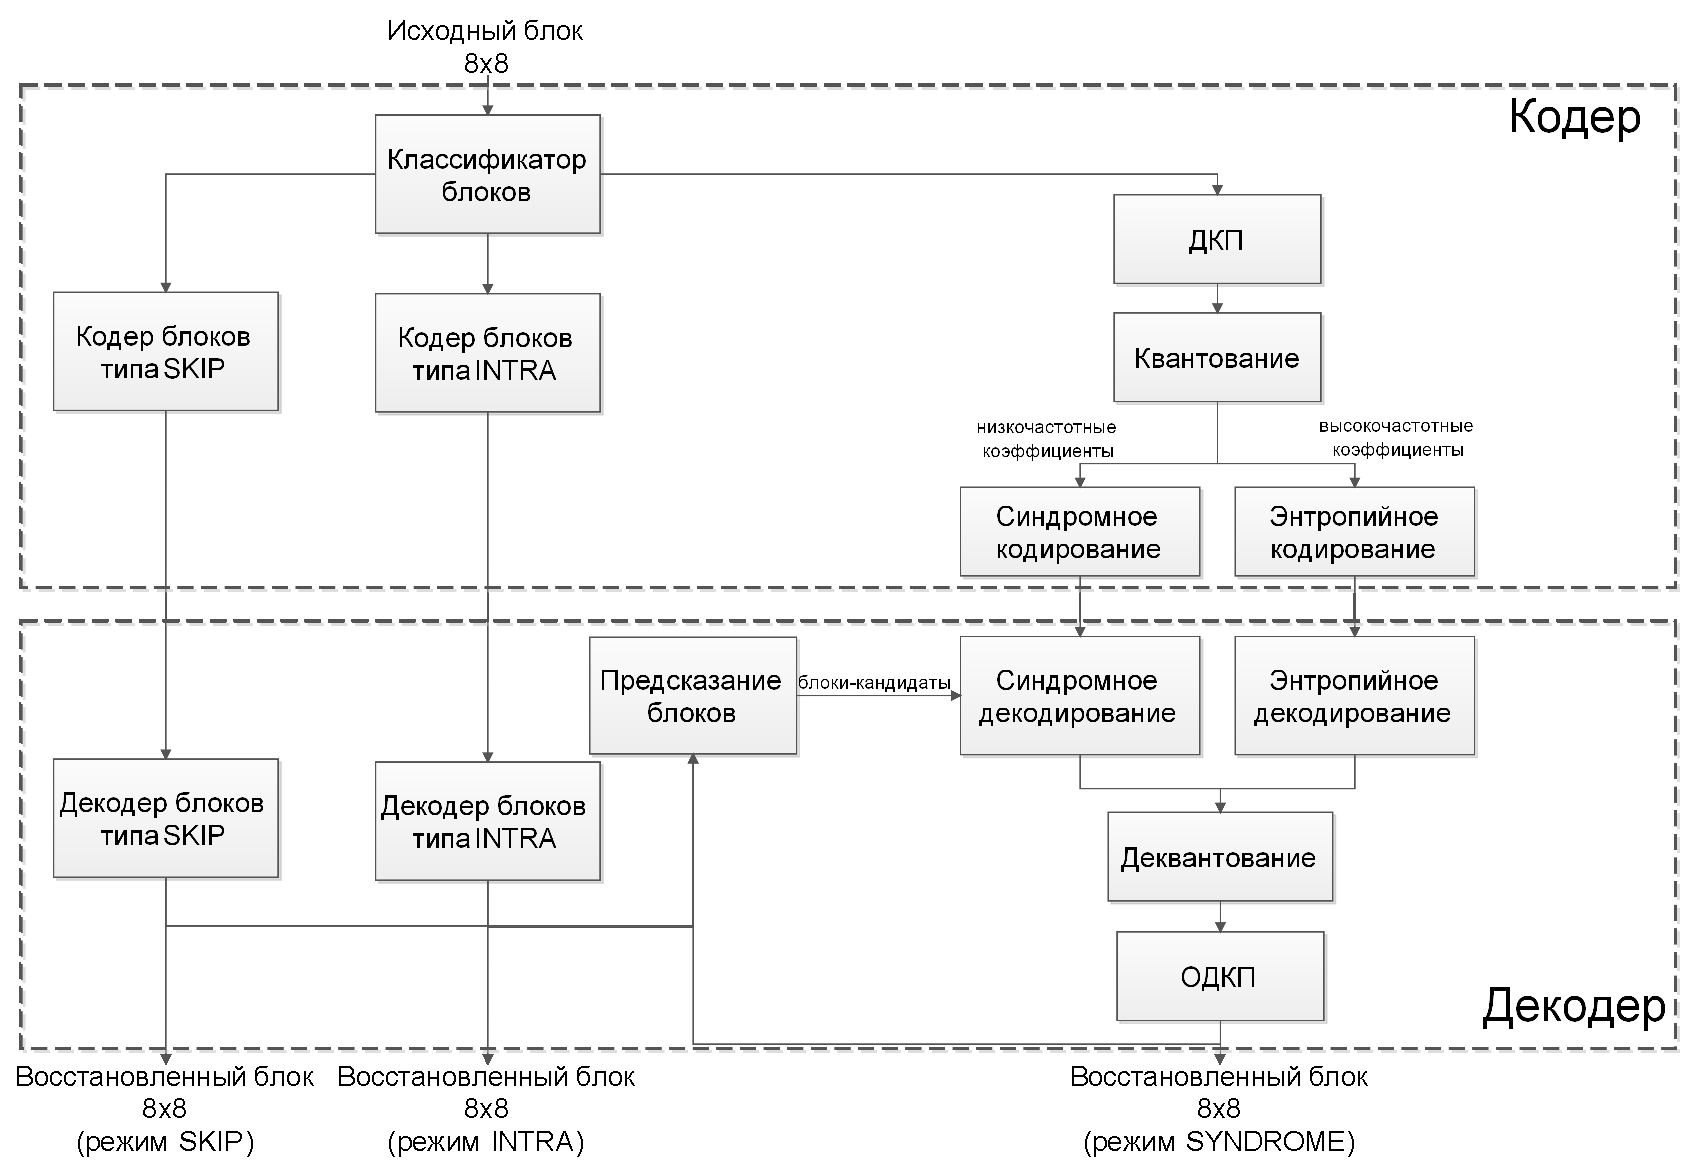
\includegraphics[width=0.9\textwidth]{Chapter1/ArchPRISM}
\caption{Типовая схема кодека, основанного на концепции PRISM}
\label{fig:ArchPRISM}
\end{center}
\end{figure}

\textbf{Кодер.} Каждый кадр видеопоследовательности разбивается на непересекающиеся блоки размером $8\times 8$ пикселей. К каждому блоку применяется дискретное косинусное преобразование и равномерное квантование. Затем блоку ставится в соответствие метка класса, которая определяет способ кодирования блока. Метка класса зависит от степени корреляции между текущим блоком, который надо сжать, и блоком предсказания из базового кадра. Процедура предсказания, в зависимости от ограничений на сложность, может работать в одном из двух режимов:

\begin{itemize}
\item блок для предсказания ищется в предыдущем обработанном кадре с использованием низкосложностной процедуры оценки движения;
\item блок для предсказания выбирается из одного из блоков, смежных с кодируемым блоком, на обрабатываемом кадре.
\end{itemize}

В зависимости от степени похожести сжимаемого блока на предсказанный блок, метка класса может принимать одно из трех значений.

\begin{itemize}
\item SKIP. В таком случае пиксели блока не кодируются (блок очень похож на предсказание).
\item INTRA. Текущий блок сжимается независимо от остальных блоков (блок совсем не похож на предсказание).
\item SYNDROME. Текущий блок сжимается с использованием вычислительно простой процедуры, основанной на распределенном кодировании (промежуточная степень схожести блока и предсказания).
\end{itemize}

Для блоков с меткой SYNDROME наиболее значимые биты квантованных спектральных коэффициентов кодируются с использованием синдромного кодирования, пример которого был приведен в подразделе~\ref{chap1:2}. В качестве помехоустойчивого кода в PRISM используется код БЧХ. Наименее значимые биты кодируются обычным энтропийным кодом.

В дополнение к сжатым данным блока кодер формирует 16-битную контрольную сумму CRC, которая, как будет описано далее, используется декодером для выбора дополнительной информации.

\textbf{Декодер.} Декодер для каждого блока формирует набор блоков-кандидатов для дополнительной информации. Блоки-кандидаты выбираются по некоторому правилу из множества уже восстановленных блоков кадра. Каждый блок из этого набора интерпретируется как сторонняя информация, и выполняется синдромное декодирование. При этом наиболее значимые биты спектральных коэффициентов декодируются с использованием синдромных бит, а наименее значимые - с использованием энтропийного декодера. Затем для каждого восстановленного блока осуществляется расчет контрольной суммы CRC по аналогии с кодером. Блок, у которого рассчитанная контрольная сумма совпадет с контрольной суммой, полученной от кодера, выбирается в качестве декодированного блока.

После декодирования блока выполняется обратное дискретное косинусное преобразование, в результате которого на стороне декодера рассчитываются пиксели восстановленного блока.

Следует отметить, что в силу того, что в схеме PRISM нет обратной связи, возможна ситуация, когда блок на стороне декодера не удастся восстановить без потерь. Подобная ситуация может возникнуть в том случае, если в наборе блоков-кандидатов не найдется блока, достаточно похожего на сжатый блок, чтобы успешно исправить все ошибки в дополнительной информации.

\section{Обоснование выбора концепции распределенного видеокодека}

Следует отметить тот факт, что концепция Стэнфорд получила большее распространение, чем PRISM. Это можно объяснить следующими наблюдениями:
\begin{itemize}
    \item схема кодека, работающего в соответствии с концепцией Стэнфорд, в большей степени, чем PRISM, соответствует существующей парадигме кодирования видеопоследовательностей, в рамках которой поток кадров разбивается на два подпотока: опорные и промежуточные;
    \item концепция Стэнфорд предоставляет большую гибкость при выборе сферы применения, т.~к. в ней присутствует возможность разнесения кодеров опорных и промежуточных кадров в пространстве/времени;
    \item кодеры, основанные на концепции Стэнфорд обладают меньшей сложностью, по сравнению с PRISM, за счет отсутствия выбора режима кодирования блоков;
    \item наличие обратной связи от кодера к декодеру обеспечивает кодекам, основанным на концепции Стэнфорд, возможность восстановления данных на стороне декодера без потерь.
\end{itemize}

В связи с этим далее в данной работе основное внимание будет уделено схемам распределенного кодирования, основанным на концепции Стэнфорд.

%Из приведенного ранее описания можно сделать вывод, что наибольшее влияние на производительность системы в целом оказывают следующие модули.
%Рассмотрим работу этих модулей на примере эталонной реализации DVC-кодека DISCOVER.

\section{Модель распределенного кодирования на базе проекта DISCOVER}
\label{chap1:5}

В 2005 году ряд исследовательских групп из нескольких Европейских университетов запустили совместный проект DISCOVER (DIStributed COding for Video sERvices)~\cite{Artigas2007}, в рамках которого была разработана базовая модель видеокодека, основанного на концепции Стэнфорд. Структурная схема распределенного кодека, работающего в соответствии с моделью DISCOVER, приведена на рисунке~\ref{fig:DiscoverScheme}. Здесь и далее будем называть данную модель~\emph{моделью кодека DISCOVER}.
 
Следует отметить, что по сравнению с концепцией Стэнфорд, модель кодека DISCOVER представляет собой существенно доработанное решение~\cite{opac-b1132593}. Одной из целей проекта была разработка методов, которые позволили бы обойти ряд конструктивных особенностей концепции Стэнфорд, не позволяющих реализовать распределенный видеокодек на практике в реальной системе. В частности, авторы DISCOVER разработали методы оценки параметров ошибок межкадрового предсказания и способы управления битовой скоростью, не требующие наличия информации о промежуточном кадре на стороне декодера. 

\begin{figure}[htbp]
\begin{center}
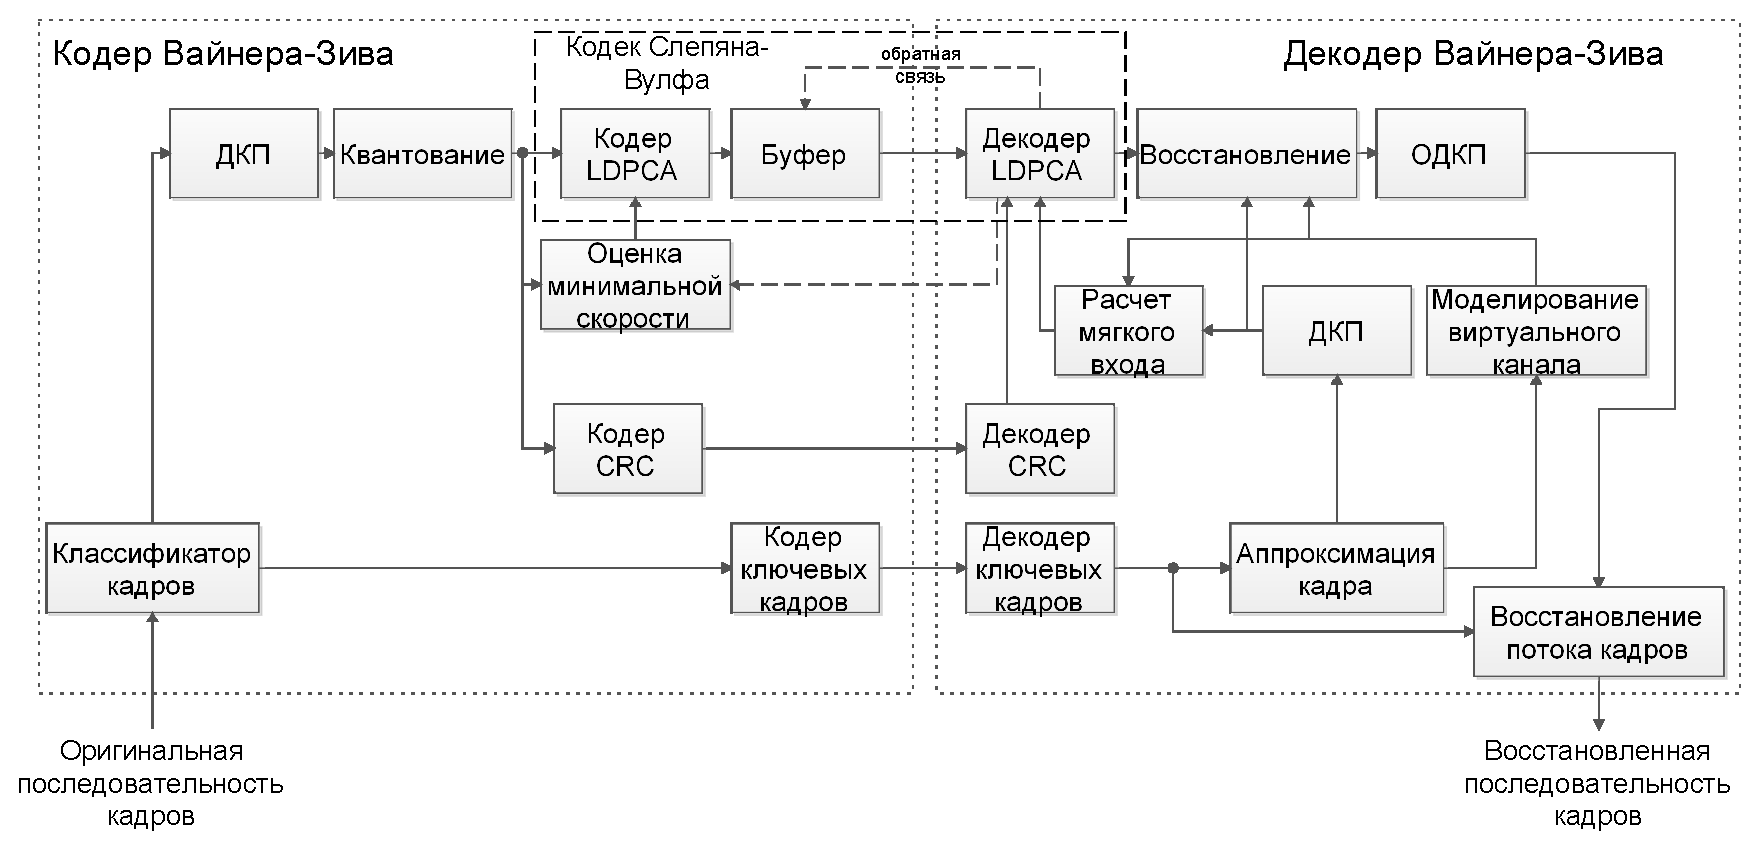
\includegraphics[width=0.9\textwidth]{Chapter1/DiscoverScheme}
\caption{Структурная схема модели кодека DISCOVER}
\label{fig:DiscoverScheme}
\end{center}
\end{figure}

Как и в концепции Стэнфорд в DISCOVER поток кадров разбивается на два подпотока: базовые (ключевые) кадры и промежуточные кадры. Ключевые кадры кодируются методом, аналогичным режиму Intra стандарта H.264~\cite{Wiegand2003} без устранения временной избыточности. Приведем описание процесса обработки промежуточных кадров в DISCOVER. Межкадровое предсказание промежуточных кадров осуществляется с помощью процедуры временной интерполяции по паре ключевых кадров. Исправление ошибок временного предсказания происходит в спектральной области. Для этого исходный кадр на стороне кодера и интерполированный кадр на стороне декодера разбиваются на непересекающиеся блоки размером $4\times4$ пикселя, которые подвергаются дискретному косинусному преобразованию (ДКП)~\cite{Khayam03thediscrete}. Спектральные коэффициенты всех блоков группируются по частотам по следующему правилу:
\begin{equation*}
G_{k,l} = \{\mathbf{T}(k+4i,l+4j)\},
\end{equation*}
где $\mathbf{T}$~--~$W\times H $ матрица спектральных коэффициентов, $\mathbf{T}(k+4i,l+4j)$ – спектральный коэффициент при паре частот $(k,l)$ для блока с номером $(i,j)$. В итоге формируется шестнадцать матриц $G_{k,l}$  размером  $(W/4) \times (H/4)$ ($W$ и $H$~--~ширина и высота кадра в пикселях соответственно), состоящих из спектральных коэффициентов при паре частот $(k,l)$, которые в дальнейшем будем называть \text{группой} (band). Затем коэффициенты в каждой группе $(k,l)$ квантуются с использованием  скалярного квантования с шагом $Q_{k,l}$. Шаг квантования определяется по диапазону значений коэффициентов в соответствующей группе~\cite{Kubasov2007}. Для различных групп используются разные методы квантования:

\begin{itemize}
\item группа с коэффициентами DC: равномерное скалярное квантование;
\item группы с коэффициентами AC: скалярное квантование с расширенной нулевой зоной.
\end{itemize}

Затем каждая группа квантованных коэффициентов разбивается на битовые плоскости $S_{k,l}^{(b)}(i,j)$, где $b$ определяет номер бита в двоичном представлении $G'_{k,l}(i,j)$. Битовые плоскости нумеруются, начиная со старшей (наиболее значимой). Обработка битовых плоскостей также начинается со старшей плоскости. На кодере каждая битовая плоскость интерпретируется как искаженное кодовое слово кода LDPCA (Low-Density Parity Check Codes with Accumulation)~\cite{Varodayan2005}. Под искажением понимается тот факт, что синдром, рассчитанный для бит плоскости, не будет является нулевым. Кодек ориентирован на работу с видеоданными форматов CIF (разрешение 352x288 пикселей) и QCIF (разрешение 176x144 пикселей), поэтому длина кода составляет $101376$ бит для CIF и $25344$ бит для QCIF. Данные параметры являются верхней оценкой для количества бит, которые декодер может запросить у кодера. Помимо бит синдрома, рассчитанных для каждой плоскости, кодер дополнительно формирует CRC (cyclic redundancy check) последовательность с использованием многочлена $f(x)=x^8+x^2+x+1$~\cite{Kubasov2007}. Эта последовательность в обязательном порядке входит в состав битового потока.

На приемной стороне декодер пытается восстановить различия в соответствующих битовых плоскостях исходных данных и результатов предсказания, используя для этого биты синдрома, сформированные кодером. Декодер DISCOVER работает по схеме с мягким входом (Soft Input), вычисляя для каждого бита кодового слова надежность~\cite{Kubasov2007}. Процедура декодирования основана на алгоритме распространения надежности. Она выполняется для каждой битовой плоскости, начиная со старшей. Для определения успешности декодирования декодер по аналогии с кодером рассчитывает контрольную сумму по информационной последовательности и сверяет её с полученной от кодера. Если CRC не совпадают, декодер запрашивает у кодера новую порцию бит синдрома и продолжает декодирование.

Использование кодов LDPCA обусловлено возможностью использования при декодировании только части бит синдрома. Таким образом, в схему DVC вводится дополнительная возможность управления битовой скоростью. В DISCOVER управление битовой скоростью осуществляется декодером при помощи канала обратной связи (feedback channel), по которому передаются запросы дополнительных бит, если декодирование с использованием имеющегося числа бит не удается.

В результате можно сделать вывод, что на эффективность устранения временной избыточности на стороне декодера и, в конечном итоге, на сжатие будут влиять следующие факторы.
\begin{itemize}
    \item Точность генерации дополнительной информации: чем меньше различий между дополнительной информацией декодера и исходными данными на стороне кодера, тем меньше проверочных бит необходимо затратить на их исправление.
    \item Эффективность исправления ошибок в дополнительной информации, на которую влияют:
    \begin{itemize}
        \item модуль оценки параметров виртуального канала: надежности символов оказывают существенное влияние на эффективность исправления ошибок с использованием корректирующих кодов;
        \item модуль помехоустойчивого кодирования: чем выше корректирующая способность кода, тем больше ошибок он позволяет исправить при фиксированной длине кода.
    \end{itemize}
\end{itemize}

Рассмотрению вопросов, связанных с этими факторами, и посвящена настоящая диссертационная работа.

\section{Области применения распределенного кодирования}

В данном подразделе перечислены основные прикладные области, в которых может применяться распределенное кодирование видеоданных~\cite{DVCApplications}. Удобно ввести в рассмотрение следующую классификацию прикладных задач в зависимости от количества источников информации:
\begin{itemize}
\item информация поступает от одного источника;
\item информация поступает от нескольких источников.
\end{itemize}

В задачах, относящихся к первому классу, кодер искусственным образом выделяет в поступающих ему на вход данных подпотоки, которые затем обрабатываются как выходы зависимых источников. Основной выигрыш от применения распределенного кодирования в таких задачах заключается в существенном уменьшении сложности процедуры сжатия на стороне кодера и, как следствие, меньших габаритах кодирующего устройства и меньшем энергопотреблении. В рамках этого класса можно выделить следующие прикладные задачи:
\begin{itemize}
\item передача данных систем видеонаблюдения с низким энергопотреблением;
\item организация мобильных видеоконференций;
\item мобильная видеопочта;
\item беспроводная капсульная эндоскопия;
\item и т. д.
\end{itemize}

В задачах, относящихся ко второму классу, как правило натуральным образом присутствует несколько зависимых источников, причем их количество может быть очень большим. Кодек в таком случае может выделить несколько основных источников, данные от которых будут использоваться как сторонняя информация при декодировании остальных источников. Использование распределенного кодирования в таком случае может, помимо уменьшения габаритов и энергопотребления, повысить надежность восстановления данных, а также отказаться от использования связей между источниками при сжатии. Ко второму классу можно отнести следующие прикладные задачи:

\begin{itemize}
\item сжатие многомерных (3D и 4D) изображений;
\item обработка информации в визуальных сенсорных сетях;
\item сжатие многовидовых видеопоследовательностей;
\item и т. д.
\end{itemize}

Однако следует отметить, что существующая инфраструктура передачи данных от мобильных видеоисточников на данный момент плохо приспособлена для использования методов распределенного кодирования на практике. В частности для систем с одним источником перенос сложности со стороны кодера на декодер требует наличия в сети специальных узлов-транскодеров, которые будут выполнять перекодирование сжатых видеопотоков в формат, обеспечивающий вычислительно простую процедуру декодирования. Тем не менее рассмотрение методов распределенного кодирования в качестве перспективной технологии является актуальной задачей.

\section{Выводы по разделу}

В качестве выводов по разделу можно отметить, что задача распределенного кодирования видеоданных представляет существенный интерес, т.~к. данный подход может найти применение во многих современных прикладных задачах, в которых требуется передать видеоинформацию от источников с ограниченными вычислительными ресурсами. В разделе приведено описание основных теоретических результатов и практических методов кодирования зависимых источников. Представлена классификация методов распределенного кодирования. Приведены основные концепции, лежащие в основе сжатия с использованием данного подхода. Далее было дано описание модели распределенного кодирования на базе проекта DISCOVER. В рамках модели выделены основные факторы, оказывающие влияние на сжатие:
\begin{itemize}
    \item точность генерации дополнительной информации;
    \item эффективность помехоустойчивого кодирования.
\end{itemize}
Исследованию этих факторов и разработке новых алгоритмов обработки видеоинформации в рамках системы распределенного кодирования и посвящена данная работа. Несмотря на то, что настоящий раздел не содержит новых результатов, его материал является вводным для последующих разделов.